%% The Supernova History of Cygnus OB2 from Gaia DR3
%% Regular A&A article -- the framing was fixed mechanically at WP9.
%%
%% BUILD:  this file needs A&A's aa.cls, which is not vendored in this
%% repository.  Fetch it from https://www.aanda.org/for-authors and place it
%% beside this file, then
%%     PYTHONPATH=../scripts python3 ../scripts/wp10_numbers.py
%%     PYTHONPATH=../scripts python3 ../scripts/wp10_figures.py
%%     latexmk -pdf main.tex
%% numbers.tex is GENERATED.  Never type a number into this file: add it to
%% scripts/wp10_numbers.py so it is read from a versioned artifact.
\documentclass{aa}

\usepackage{graphicx}
\usepackage{txfonts}
\usepackage{amsmath}
\usepackage[colorlinks,citecolor=blue,urlcolor=blue,linkcolor=blue]{hyperref}

% ---------------------------------------------------------------
% manuscript/numbers.tex -- GENERATED, DO NOT EDIT BY HAND.
% Produced by scripts/wp10_numbers.py from versioned artifacts
% resolved through scripts/wp10_inputs.py.  Regenerate with:
%   PYTHONPATH=scripts python3 scripts/wp10_numbers.py
% Every macro's source file is given in the trailing comment.
% ---------------------------------------------------------------
\newcommand{\Cfour}{0.854}% wp9_verdict.csv
\newcommand{\Conehi}{0.861}% wp9_verdict.csv
\newcommand{\Conelo}{0.379}% wp9_verdict.csv
\newcommand{\Cthree}{1.000}% wp9_verdict.csv
\newcommand{\NSN}{8.43}% wp7_ledger.csv
\newcommand{\NSNA}{4.17}% wp7_ledger.csv
\newcommand{\NSNB}{4.26}% wp7_ledger.csv
\newcommand{\NSNC}{0.00}% wp7_ledger.csv
\newcommand{\NSNallfactor}{14.9}% wp7_ledger.csv
\newcommand{\NSNalllo}{1.93}% wp7_ledger.csv
\newcommand{\NSNatSix}{38.2}% wp7_age_sensitivity.csv
\newcommand{\NSNdrophi}{4.24}% wp7_ledger.csv
\newcommand{\NSNdroplo}{1.93}% wp7_ledger.csv
\newcommand{\NSNheadbranches}{36}% wp7_ledger.csv
\newcommand{\NSNheadfactor}{5.1}% wp7_ledger.csv
\newcommand{\NSNheadhi}{28.7}% wp7_ledger.csv
\newcommand{\NSNheadlo}{5.63}% wp7_ledger.csv
\newcommand{\NSNhi}{11}% wp7_ledger.csv
\newcommand{\NSNlo}{5}% wp7_ledger.csv
\newcommand{\NSNmedian}{8}% wp7_ledger.csv
\newcommand{\Nlabelled}{1,331}% wp2_subgroup_labels.parquet
\newcommand{\Nmembers}{1,392}% wp2_members.parquet
\newcommand{\NmembersAll}{2,112}% wp2_members.parquet
\newcommand{\NsubA}{476}% wp2_subgroup_labels.parquet
\newcommand{\NsubB}{426}% wp2_subgroup_labels.parquet
\newcommand{\NsubC}{429}% wp2_subgroup_labels.parquet
\newcommand{\Pone}{0.9997}% wp7_ledger.csv
\newcommand{\Ppermhi}{0.854}% wp9_verdict.csv
\newcommand{\Ppermlo}{0.727}% wp9_verdict.csv
\newcommand{\Precent}{0.552}% wp7_ledger.csv
\newcommand{\Precentheadhi}{0.889}% wp7_ledger.csv
\newcommand{\Precentheadlo}{0.411}% wp7_ledger.csv
\newcommand{\PverdictTwoThreehi}{0.474}% wp9_verdict.csv
\newcommand{\PverdictTwoThreelo}{0.323}% wp9_verdict.csv
\newcommand{\PverdictTwoThreen}{18}% wp9_verdict.csv
\newcommand{\PverdictTwohi}{0.735}% wp9_verdict.csv
\newcommand{\PverdictTwolo}{0.593}% wp9_verdict.csv
\newcommand{\PverdictTwon}{18}% wp9_verdict.csv
\newcommand{\Pverdictbranches}{36}% wp9_verdict.csv
\newcommand{\Pverdicthi}{0.735}% wp9_verdict.csv
\newcommand{\Pverdictlo}{0.323}% wp9_verdict.csv
\newcommand{\Pverdictmed}{0.533}% wp9_verdict.csv
\newcommand{\Pverdictsixhi}{0.250}% wp9_verdict.csv
\newcommand{\Pverdictsixlo}{0.142}% wp9_verdict.csv
\newcommand{\ageA}{4.00}% wp4_wp5_age_reconciliation.csv
\newcommand{\ageB}{4.09}% wp4_wp5_age_reconciliation.csv
\newcommand{\ageC}{2.52}% wp4_wp5_age_reconciliation.csv
\newcommand{\ageShiftB}{0.54}% wp4_wp5_age_reconciliation.csv
\newcommand{\ageSpread}{1.57}% wp4_wp5_age_reconciliation.csv
\newcommand{\ageZeroBelow}{3.00}% wp7_age_sensitivity.csv
\newcommand{\ageumsA}{3.98}% wp4_wp5_age_reconciliation.csv
\newcommand{\ageumsB}{3.55}% wp4_wp5_age_reconciliation.csv
\newcommand{\ageumsC}{2.51}% wp4_wp5_age_reconciliation.csv
\newcommand{\alphaCells}{18}% wp5_alpha_plausibility_execution.json
\newcommand{\alphaSixChi}{10.80}% wp5_alpha_plausibility_execution.json
\newcommand{\alphaSixWins}{1}% wp5_alpha_plausibility_execution.json
\newcommand{\alphaThreeChi}{6.86}% wp5_alpha_plausibility_execution.json
\newcommand{\bhSafeCut}{30}% wp7_alpha_headline_adoption_outcome.json
\newcommand{\binaryBracket}{30}% wp7_binary_bound_execution.json
\newcommand{\binaryHi}{10.96}% wp7_binary_bound_execution.json
\newcommand{\binaryLo}{5.90}% wp7_binary_bound_execution.json
\newcommand{\binaryRatio}{5}% wp7_binary_bound_execution.json
\newcommand{\binarySpan}{5.1}% wp7_binary_bound_execution.json
\newcommand{\bpassRatioHi}{0.73}% wp7_binary_bound_execution.json
\newcommand{\bpassRatioLo}{0.72}% wp7_binary_bound_execution.json
\newcommand{\branchSpan}{23.1}% wp7_binary_bound_execution.json
\newcommand{\branchesPassing}{40}% wp5_repair_v6_gate.json
\newcommand{\branchesTotal}{54}% wp5_repair_v6_gate.json
\newcommand{\closingAlpha}{2.25}% derived, wp6_closure_repair_v7.csv
\newcommand{\closureA}{0.865}% wp6_closure_repair_v7.csv
\newcommand{\closureB}{1.068}% wp6_closure_repair_v7.csv
\newcommand{\closureC}{1.360}% wp6_closure_repair_v7.csv
\newcommand{\closureCells}{18}% derived, wp6_closure_repair_v7.csv
\newcommand{\closureCellsInside}{18}% derived, wp6_closure_repair_v7.csv
\newcommand{\closureExcess}{6.7}% wp6_closure_repair_v7.csv
\newcommand{\closureMedian}{1.067}% wp6_closure_repair_v7.csv
\newcommand{\controlYield}{3.7}% table2_wp2_gate.md
\newcommand{\firstSN}{1.30}% wp7_rsn_curves.csv
\newcommand{\fracBelowFiftyTwo}{19}% wp7_alpha_headline_branch_sets.csv
\newcommand{\gammaCygni}{7.7}% wp8_crosschecks.csv
\newcommand{\ignorance}{0.077}% derived, wp7_rsn_curves.csv
\newcommand{\kA}{1,734}% wp5_imf_normalization_repair_v7.parquet
\newcommand{\kB}{1,647}% wp5_imf_normalization_repair_v7.parquet
\newcommand{\kC}{1,894}% wp5_imf_normalization_repair_v7.parquet
\newcommand{\livingMembers}{295.4}% wp6_ledger_execution.json
\newcommand{\livingOrphans}{27}% wp6_ledger_execution.json
\newcommand{\livingRetained}{322.4}% derived, wp6_ledger_execution.json
\newcommand{\livingTotal}{380.6}% wp6_ledger_execution.json
\newcommand{\massPrimaries}{2.42}% wp5_association_mass_reconciliation.csv
\newcommand{\massPrimariesHalf}{1.75}% wp5_association_mass_reconciliation.csv
\newcommand{\massTotal}{2.92}% wp5_association_mass_reconciliation.csv
\newcommand{\massVsWright}{1.47}% wp5_association_mass_reconciliation.csv
\newcommand{\measurementFactor}{7}% derived, wp7_ledger.csv and wp7_rsn_curves.csv
\newcommand{\minProgenitor}{33.9}% wp7_alpha_headline_branch_sets.csv
\newcommand{\minTurnoffAll}{33.9}% wp7_alpha_headline_branch_sets.csv
\newcommand{\minTurnoffCoeval}{45.4}% wp7_alpha_headline_branch_sets.csv
\newcommand{\ourDistance}{1.62}% wp8_crosschecks.csv
\newcommand{\pulsarAge}{0.960}% wp8_crosschecks.csv
\newcommand{\pulsarIslands}{0}% wp8_crosschecks.csv
\newcommand{\pulsarPone}{0.9997}% wp8_crosschecks.csv
\newcommand{\railB}{53}% wp4_wp5_age_reconciliation.csv
\newcommand{\railtopB}{4.26}% wp4_wp5_age_reconciliation.csv
\newcommand{\rateNow}{8.0}% wp7_rsn_curves.csv
\newcommand{\runawayFraction}{14.6}% derived, wp6_ledger_execution.json
\newcommand{\runawaysBinned}{58.2}% wp6_ledger_execution.json
\newcommand{\runawaysCorrected}{54.9}% wp6_ledger_execution.json
\newcommand{\runawaysRaw}{119}% wp6_ledger_execution.json
\newcommand{\snRatioB}{1.92}% wp4_wp5_age_reconciliation.csv
\newcommand{\snrExpected}{0.80}% wp8_crosschecks.csv
\newcommand{\spreadAlpha}{0.264}% wp9_sensitivity.csv
\newcommand{\spreadDelta}{0.043}% wp9_sensitivity.csv
\newcommand{\spreadFamily}{0.045}% wp9_sensitivity.csv
\newcommand{\spreadRv}{0.065}% wp9_sensitivity.csv
\newcommand{\tlast}{86}% wp7_ledger.csv
\newcommand{\turnoffA}{58}% wp4_wp5_age_reconciliation.csv
\newcommand{\turnoffB}{56}% wp4_wp5_age_reconciliation.csv
\newcommand{\turnoffC}{279}% wp4_wp5_age_reconciliation.csv


\begin{document}

\title{The supernova history of Cygnus~OB2 from \textit{Gaia}~DR3}
\subtitle{A probabilistic ledger of massive-star deaths from a homogeneous census}

\author{
  V.~Voitsekhovskyi\inst{1}
  \and
  (co-authors to be confirmed)\inst{1}
}
\institute{Affiliation to be completed \email{jstvdk@gmail.com}}

\date{Received ---; accepted ---}

\abstract
% context
{Cygnus~OB2 is one of the most massive young stellar associations in the
Galaxy, and its past supernovae shape everything around it: the mechanical
energy of the superbubble, the compact-remnant population, the radioactive
$^{26}$Al budget, and the viability of every interpretation of the region's
high-energy emission that invokes a recent explosion. Yet its supernova history
has never been measured from a homogeneous census --- existing numbers are
population-synthesis estimates built on heterogeneous literature inputs.}
% aims
{We measure the supernova history of Cygnus~OB2 as a population property ---
how many core-collapse supernovae it has produced, their timeline, and the time
since the most recent --- independently of any single interpretation of the
region's high-energy emission.}
% methods
{From \textit{Gaia}~DR3 astrometry and photometry joined to 2MASS and to a
literature spectroscopic census, we build a probabilistic member list and its
kinematic substructure, fit per-star extinctions against a spectroscopically
anchored spatial prior, derive subgroup ages and per-star masses from two
isochrone families, and normalize the initial mass function by a
response-aware Poisson fit to completeness-corrected star counts between 2 and
8\,$M_\odot$. Supernovae are then counted by stellar-evolution turnoff in a
Monte Carlo over $2\times10^{6}$ population realizations per branch. Discrete
modelling choices --- isochrone family, extinction law, IMF slope,
star-formation duration, explodability --- are carried as branches and never
averaged. Every marker comparison was pre-registered before it was computed.}
% results
{Cygnus~OB2 resolves into three kinematic subgroups of \ageA, \ageB\ and \ageC\
Myr: two older and one younger. It has produced $N_{\rm SN} = \NSN$ supernovae
on the baseline branch (median \NSNmedian, 68\% [\NSNlo, \NSNhi]), with a
carried range of \NSNheadlo--\NSNheadhi\ across \NSNheadbranches\ branches, the
first \firstSN\,Myr ago and the most recent probably within the last
100\,kyr ($P = \Precent$). The entire budget lies above $\bhSafeCut\,M_\odot$:
for any black-hole threshold at or below that mass the ledger returns exactly
zero on every branch, so the result is conditional on whether very massive
stars explode at all. PSR~J2032+4127, whose companion is a star in our own
census, settles that branch --- a neutron star requires a successful explosion
--- and its age and kinematics agree with a ledger built without looking at it.
As one application of the ledger, the probability that Cygnus~OB2 supplied a
supernova of the age, progenitor type and location that supernova-driven models
of the Cygnus $\gamma$-ray cocoon require is
$P = \Pverdictlo$--\Pverdicthi\ (median \Pverdictmed), supported on
\PverdictTwon\ of \PverdictTwon\ branches at $\alpha = 2.0$ and on none at
$\alpha = 2.3$.}
% conclusions
{Cygnus~OB2 is an active supernova factory whose entire budget is carried by
its most massive stars. The supernova-driven cocoon scenario is supported under
those models' own permissive age allowance ($P = \Ppermlo$--\Ppermhi) and
unresolved at their preferred $\sim$50\,kyr, hinging almost entirely on the
high-mass IMF slope --- an axis \textit{Gaia}~DR4 will not settle, but a second
association analysed identically would.}

\keywords{stars: massive -- open clusters and associations: individual:
Cygnus OB2 -- supernovae: general -- gamma rays: ISM -- astrometry}

\maketitle

%===============================================================
\section{Introduction}\label{sec:intro}

Cygnus~OB2 is one of the most massive young stellar associations in the Galaxy
--- tens of O stars, three Wolf--Rayet stars and a young pulsar
\citep{wright2015, berlanas2020} --- and the engine of the Cygnus~X region.
Much of what is astrophysically interesting around it traces back to a single
unmeasured population property: how many of its stars have already died, and
when. The supernova count and timeline set the mechanical energy injected into
the superbubble, the expected compact-remnant population, the radioactive
$^{26}$Al budget, and the plausibility of every interpretation of the region's
high-energy emission that invokes a recent explosion.

That last dependence has become acute. The $\gamma$-ray cocoon around
Cygnus~OB2, detected from GeV to hundreds of TeV, is the clearest Galactic
PeVatron candidate, and the proposed accelerators span the association's
collective winds, a supernova exploding into the cavity those winds have carved
\citep{harer2025, suppresseddiffusion2026}, and --- since LHAASO's detection of
a variable ultra-high-energy source coincident with Cygnus~X-3 --- a
microquasar \citep{cygx3pevatron2026}. The field also hosts high-energy sources
in their own right: the $\gamma$~Cygni supernova remnant and the pulsar
PSR~J2032+4127 with its wind nebula. These candidates are not mutually
exclusive, but they place different demands on the stellar population, and the
supernova-driven class places the sharpest one: \citet{harer2025} require an
event of $3$--$5\times10^{51}$\,erg from a stripped-envelope progenitor, inside
the cavity, within the last few tens to few hundreds of kiloyears. Cygnus~OB2
contains three Wolf--Rayet stars, tens of supergiants and a young pulsar, so
supernovae have surely occurred; but ``surely at least one'' is not the same
statement as ``one within the last 100\,kyr'', and to date the stronger
statement has been supported by plausibility arguments rather than by a census.

The stellar side of the problem is tractable. If the present-day mass function
of an association is measured where it is complete, the initial mass function
can be normalized there and extrapolated above the turnoff, and the stars that
are missing from the upper main sequence are the ones that have died. This is
the deficit method of \citet{fuchs2006} and \citet{zucker2022}, and
\textit{Gaia}~DR3 makes it possible to apply it to Cygnus~OB2 with membership,
distance and extinction all derived from the same homogeneous data set rather
than assembled from the literature.

Prior estimates exist and disagree in ways that trace to their inputs rather
than to their methods: \citet{knodlseder2002} and \citet{martin2010} modelled
the Cygnus complex as a whole, and \citet{menchiari2024} adopt a fixed
association mass and predict $7\pm2.5$ supernovae at 3\,Myr and $26\pm5$ at
5\,Myr --- a factor of four spanned by a 2\,Myr change in an assumed age. Any
new number is only useful if it comes with the machinery to say why it differs
from the old ones.

This paper supplies that: a measurement of the supernova history of Cygnus~OB2
as a property of its stellar population, made prior to --- and independently
of --- any particular interpretation of the high-energy emission.
Section~\ref{sec:data} describes the data, Sect.~\ref{sec:method} the chain
from membership to the supernova ledger, and Sect.~\ref{sec:results} the
results and the external cross-checks. Only then, in
Sect.~\ref{sec:discussion}, is the measured ledger confronted with the
supernova-driven interpretation of the cocoon, alongside what the answer does
and does not settle. Three
choices govern everything and are stated here rather than buried: discrete
modelling choices are \emph{carried as branches and never averaged}; every
comparison against an independent supernova marker was \emph{pre-registered}
before it was computed; and results that failed are reported as failed.

%===============================================================
\section{Data}\label{sec:data}

\subsection{\textit{Gaia} DR3 and 2MASS}

Two \textit{Gaia}~DR3 queries define the working samples: a narrow box
($l \in [77\degr, 83\degr]$, $b \in [-1\fdg5, +4\degr]$) for the census, and a
wide box ($l \in [72\degr, 88\degr]$, $b \in [-5\degr, +8\degr]$) for runaway
traceback. Parallaxes were selected in $[0.35, 1.1]$\,mas and $G < 19$ ---
deliberately generous, because the selection is refined by clustering rather
than by cuts. Parallax zero-points follow \citet{lindegren2021}. Near-infrared
photometry comes from the official \textit{Gaia} $\times$ 2MASS cross-match.

\subsection{Spectroscopic anchors and supernova markers}

The brightest O stars have unreliable or missing \textit{Gaia} astrometry, so
they cannot be allowed to fall out of the census silently. A merged anchor
table carries spectral types and, where available, effective temperatures from
\citet{wright2015}, \citet{berlanas2019, berlanas2020} and the Galactic O-Star
Catalog; the spectral reclassification of the association's B0 population by
\citet{fastrotators2025} postdates our freeze and should be folded in at the
DR4 rerun; all \NmembersAll{} rows of the \textit{Gaia}-based member catalogue are
supplemented by these anchors, which are exempt from the astrometric quality
cuts and are treated individually.

Independent supernova markers --- PSR~J2032+4127 from the ATNF catalogue,
$\gamma$~Cygni (G78.2+2.1) from Green's supernova-remnant catalogue, and the
INTEGRAL $^{26}$Al measurements of the Cygnus region --- were frozen at the
data-acquisition stage, \emph{before} any ledger existed. Their comparison
statistics were fixed in a pre-registration written before the ledger was run.

%===============================================================
\section{Method}\label{sec:method}

\subsection{Membership and substructure}\label{sec:membership}

Members are identified by Gaussian-mixture clustering in
$(l, b, \mu_{\alpha*}, \mu_\delta)$, with membership probabilities from a Monte
Carlo over each star's full astrometric covariance. Parallax is deliberately
\emph{excluded} as a clustering feature: the member sample forms a single
population at $\ourDistance$\,kpc with an intrinsic depth of $\sim$45\,pc,
which DR3 parallaxes cannot resolve, so including it would manufacture
structure rather than find it. The number of components was accepted on
seed stability rather than on an information criterion; only $k = 3$ is stable
across 50 deterministic seeds.

The gate is conjunctive and was applied before any downstream work: recall of
\citet{berlanas2019} spectroscopic members, the yield of three control fields
processed identically, the member count, the spatial compactness of the
recovered structure, and a no-percolation criterion. All were met. Of
\NmembersAll{} catalogue rows, \Nmembers{} have $P > 0.5$ and \Nlabelled{}
carry a subgroup label: Cyg~OB2-A (\NsubA), Cyg~OB2-B (\NsubB) and
Cyg~OB2-C (\NsubC).

\begin{figure*}[t]
\centering
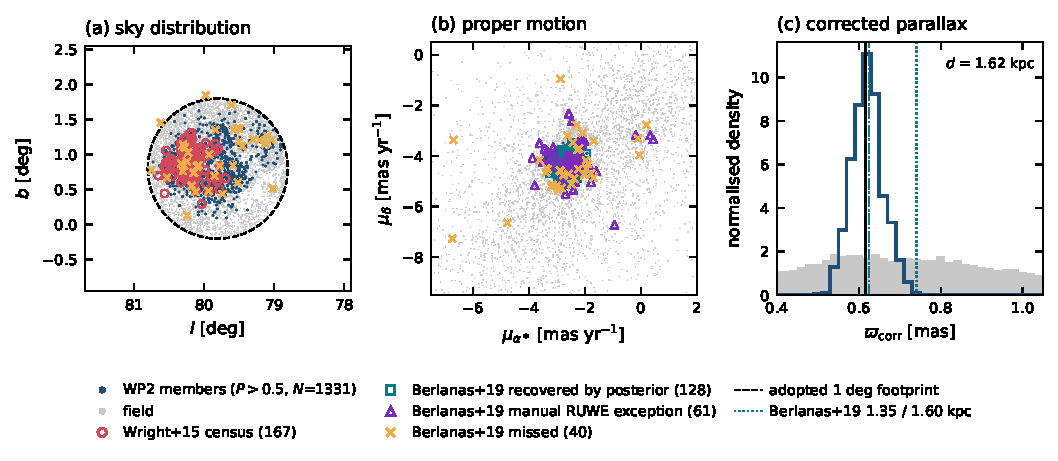
\includegraphics[width=\textwidth]{../figures/paper/fig1_membership_literature.pdf}
\caption{Membership and substructure. Sky distribution and proper-motion plane
of the \Nmembers{} members with $P > 0.5$, coloured by kinematic subgroup, with
the \citet{berlanas2019} and \citet{wright2015} literature samples overlaid.
Parallax is deliberately excluded as a clustering feature
(Sect.~\ref{sec:membership}).}
\label{fig:membership}
\end{figure*}

\begin{figure}[t]
\centering
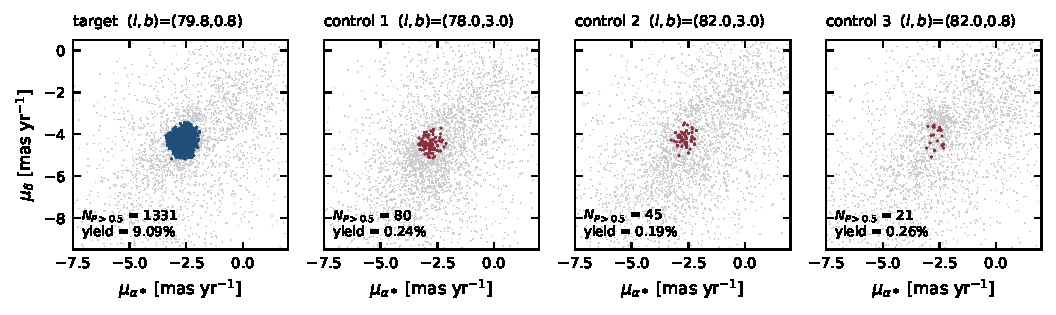
\includegraphics[width=\columnwidth]{../figures/paper/fig2_control_fields.pdf}
\caption{The false-positive rate, measured rather than assumed. Three control
fields at matched Galactic latitude were processed through the identical
selection, clustering and membership model; their yield is \controlYield\% of the association field's.}
\label{fig:control}
\end{figure}

We do \emph{not} confirm the two-distance structure of \citet{berlanas2019}
within the member sample, and we state the limit of that non-confirmation
precisely: parallax was a selection feature, so a foreground group would have
been removed before the test ran. The correct claim is that there is no
evidence of two distances \emph{among the members we select}, not that the
foreground group does not exist. A parallax-blind membership test is the only
way to settle it and is deferred.

\subsection{Extinction and ages}\label{sec:extinction}

Differential extinction is the Cygnus problem, and a single regional $A_V$ is
inadmissible. Anchors receive $A_V$ from fixed-$T_{\rm eff}$ intrinsic colours,
which avoids the temperature--extinction degeneracy that broadband photometry
suffers for hot stars; all other members are fitted against reddened synthetic
photometry from the same isochrone families used for the ages, with an
anchor-informed spatial prior. That prior's mean is a simple-kriging estimate
using a variogram fitted to the anchors themselves, and its width is the
unconditional variogram sigma --- one internally consistent object, where an
earlier version widened the width for distant anchors while still centring on
them at full weight.

Subgroup ages come from the de-reddened colour--magnitude diagrams with an
unresolved-binary population included in the likelihood rather than clipped
away. These upper-main-sequence ages (\ageumsA, \ageumsB, \ageumsC\,Myr) are
\emph{the prior}, not the adopted values: the ages used downstream are the
counts-based ages of Sect.~\ref{sec:imf}.

\subsection{IMF normalization}\label{sec:imf}

The normalization $k$ is fitted per subgroup by a Poisson likelihood over mass
bins between 2 and 8\,$M_\odot$, against a forward model that convolves the
assumed IMF with a completeness response measured by injecting synthetic stars
into the real field and recovering them through the actual selection. The
response, not a scalar completeness, is the correct object: the mass estimator
has 22--25\% scatter, so it scatters stars across bin edges and across the
window boundaries in both directions.

The truth-side age is marginalized jointly with $k$. The forward response is a
mixture over nine age nodes drawn from the CMD posterior, reweighted by the
Poisson likelihood of the observed counts with $k$ integrated out analytically.
This produces a \emph{counts-based} age --- the age at which the injected
population reproduces the observed mass function --- which is what the ledger
consumes. On the baseline branch these are \ageA, \ageB\ and \ageC\,Myr, with
normalizations $k = \kA$, \kB\ and \kC.

Only Cyg~OB2-B moves materially between the two age definitions, by
$+\ageShiftB$\,Myr, and that shift is worth a factor \snRatioB\ in B's supernova
count --- which is why both are reported and labelled. B's counts-based
posterior concentrates \railB\% of its weight on the topmost of its nine nodes,
so its age is bounded from below by the data and from above by the prior grid;
its supernova contribution is correspondingly a lower bound
(Sect.~\ref{sec:systematics}).

\begin{figure*}[t]
\centering
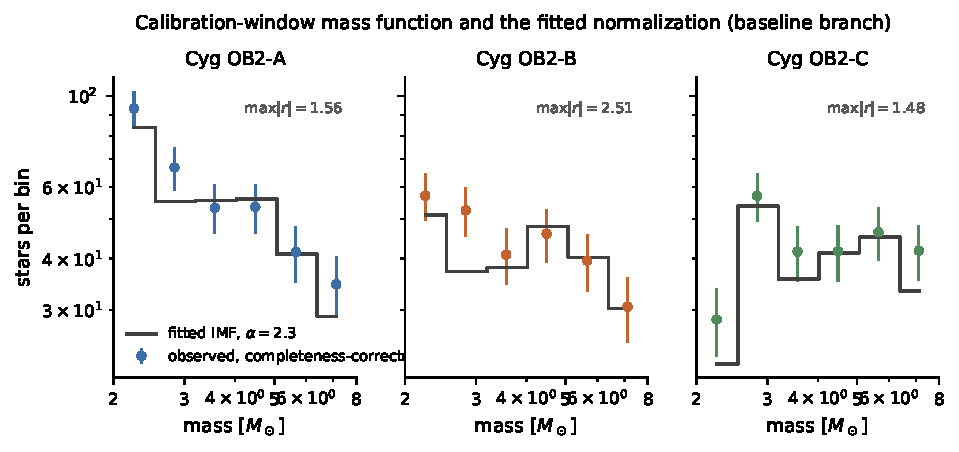
\includegraphics[width=\textwidth]{../figures/paper/fig3_mass_function.pdf}
\caption{The calibration-window mass function per subgroup on the baseline
branch, with the fitted normalization overlaid. The fit is a Poisson likelihood
against a forward model that convolves the assumed IMF with the measured
completeness response, not against a completeness-divided histogram. Worst
Pearson residuals are annotated.}
\label{fig:massfunction}
\end{figure*}

\subsection{Census closure and runaways}\label{sec:closure}

The closure test compares the number of living stars above 8\,$M_\odot$
predicted by the normalization against the number observed. It is an
\emph{out-of-sample} test: $k$ is fitted from 2--8\,$M_\odot$ counts and the
$>8\,M_\odot$ census never enters that likelihood. Both sides are computed with
the same forward response, integrated with no lower cut-off, because the
observed side counts every member's $P(M > 8\,M_\odot)$ whatever its true mass.

Runaways are recovered from the wide box by tracing proper motions backwards
over the subgroup age windows, with the association's systemic motion
subtracted --- Cygnus~OB2's bulk motion is larger than a typical ejection
signature, so absolute proper motions measure drift rather than ejection. The
false-positive rate is measured per separation bin from control fields, in the
same spirit as recent Gaia runaway searches in other associations
\citep{velob1runaways2026}.

\subsection{The supernova ledger}\label{sec:ledger}

For each branch and each of $2\times10^{6}$ iterations we draw a paired
$(k, \mathrm{age})$ sample from the joint posterior --- paired, because the two
are correlated through the fit --- draw a star-formation duration, sample a
discrete stellar population from the IMF conditioned on the calibration-window
counts, and ask which stars have passed the turnoff. Supernovae are then those
deaths that satisfy the explodability branch.

Runaways do \emph{not} enter $N_{\rm SN}$. They are living stars below the
turnoff, so they change neither $k$, which is fitted below 8\,$M_\odot$, nor the
turnoff mass. What they bound is location, not number
(Sect.~\ref{sec:crosschecks}).

\subsection{Branches, and what is never averaged}\label{sec:branches}

Isochrone family \{PARSEC, MIST\} $\times$ extinction law
$R_V \in \{3.0, 3.1, 3.5\}$ $\times$ IMF slope $\alpha \in \{2.0, 2.3, 2.6\}$
$\times$ star-formation duration $\delta \in \{0, 1, 2\}$\,Myr $\times$
explodability \{all explode, islands of implosion\}. The baseline branch is
PARSEC, $R_V = 3.1$, $\alpha = 2.3$, $\delta = 0$, all explode.
\branchesPassing\ of \branchesTotal\ mass-function fits pass the residual gate;
no branch is ever dropped for failing it, and the failures are reported by
their concentration in the $R_V = 3.5$ and $\alpha = 2.6$ corners.

The \emph{headline} branch set excludes $\alpha = 2.6$. The criterion is the
calibration-window $\chi^2$, an internal gate statistic fixed long before the
ledger existed, on which $\alpha = 2.6$ is the best fit in \alphaSixWins\ of
\alphaCells\ cells and has the worst median ($\chi^2 = \alphaSixChi$ against
\alphaThreeChi\ for $\alpha = 2.3$). The census closure agrees independently but was deliberately
\emph{not} used to make this choice, so that it remains available as an
out-of-sample validation of the extrapolation (Sect.~\ref{sec:closure-result}).
$\alpha = 2.6$ is reported throughout with its own numbers
($N_{\rm SN} = \NSNdroplo$--\NSNdrophi, $P_{\rm verdict} = \Pverdictsixlo$--%
\Pverdictsixhi) and is never deleted.

%===============================================================
\section{Results}\label{sec:results}

\subsection{A revised star-formation history}\label{sec:sfh}

Cygnus~OB2 is not coeval. Its three kinematic subgroups have counts-based ages
of \ageA, \ageB\ and \ageC\,Myr --- \textbf{two older subgroups and one
younger}, with a total spread of \ageSpread\,Myr. This differs from the
structure the same pipeline returned before the extinction prior was corrected,
which read as one older subgroup and two younger; the change followed a
pre-registered fix whose four predictions were confirmed in advance, with
Cyg~OB2-B moving by $+0.73$\,Myr and A and C by $0.000$\,Myr.

The supernova timeline follows directly. A and B supply the entire budget --- their turnoffs stand at \turnoffA\ and
\turnoffB\,$M_\odot$ --- while Cyg~OB2-C's sits at \turnoffC\,$M_\odot$, still
above the IMF's upper limit, so it has lost no stars at all.

The wider envelope across both retained age indicators is 2.25--5.67\,Myr, and
that --- not the spread between the three central values --- is the age
uncertainty everything downstream inherits (Fig.~\ref{fig:age}).

\subsection{The ledger}\label{sec:ledger-result}

On the baseline branch Cygnus~OB2 has produced

\begin{equation}
N_{\rm SN} = \NSN \quad (\text{median } \NSNmedian,\ 68\%\ [\NSNlo, \NSNhi]),
\end{equation}

comprising \NSNA\ from Cyg~OB2-A, \NSNB\ from Cyg~OB2-B and exactly \NSNC\ from
Cyg~OB2-C. The probability that at least one supernova has occurred is
\Pone; the probability that the most recent one falls within the last 100\,kyr
is \Precent, and the median time since it is \tlast\,kyr. The first explosion
was \firstSN\,Myr ago and the rate has been roughly flat at
$\rateNow$\,Myr$^{-1}$ since (Fig.~\ref{fig:rsn}).

\textbf{The number is not \NSN.} Across the \NSNheadbranches\ headline branches
the total spans \NSNheadlo--\NSNheadhi, a factor of \NSNheadfactor; including
$\alpha = 2.6$ it reaches down to \NSNalllo, a factor of \NSNallfactor. The
branch spread \emph{is} the uncertainty; the Poisson interval on any one branch
is the smaller part of it. The same is true of the recent-supernova
probability, which spans \Precentheadlo--\Precentheadhi\ across the headline
branches. We quote the baseline value with its carried range
beside it and never an average across branches, which for a set that carries no
probability weights would not be a posterior summary.

\begin{figure}[t]
\centering
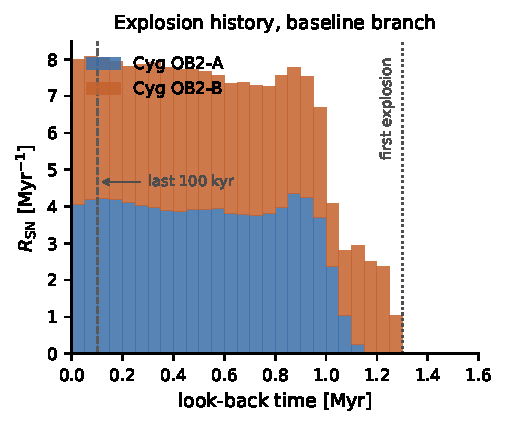
\includegraphics[width=\columnwidth]{../figures/paper/fig4_rsn_history.pdf}
\caption{The explosion history $R_{\rm SN}(t)$ on the baseline branch, stacked
by subgroup. Cyg~OB2-C contributes nothing: its turnoff has not yet fallen
below the IMF's upper limit. The rate is roughly flat since the first explosion
\firstSN\,Myr ago, which is why $P(t_{\rm last} < 100\,$kyr$) = \Precent$.}
\label{fig:rsn}
\end{figure}

\begin{figure}[t]
\centering
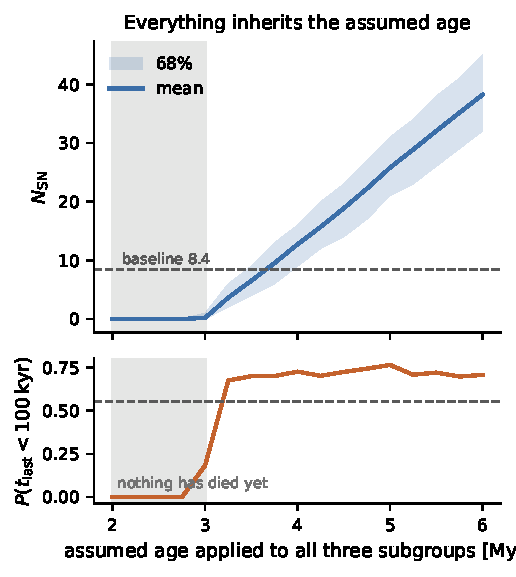
\includegraphics[width=\columnwidth]{../figures/paper/fig5_age_sensitivity.pdf}
\caption{The mandatory honesty plot: $N_{\rm SN}$ and $P(t_{\rm last} <
100\,$kyr$)$ as functions of a common assumed age applied to all three
subgroups. Below \ageZeroBelow\,Myr the turnoff has not crossed the IMF ceiling
and nothing has died; above it the count rises by roughly 12 supernovae per Myr
of assumed age, reaching \NSNatSix\ at 6\,Myr. Everything this paper reports inherits the ages of
Sect.~\ref{sec:imf}, and this is how that dependence is disclosed rather than
absorbed.}
\label{fig:age}
\end{figure}

\subsection{The whole budget lies above $\bhSafeCut\,M_\odot$}\label{sec:structural}

Every star that has died in Cygnus~OB2 is very massive. On the baseline branch
the lowest progenitor that exploded is $52\,M_\odot$, and the lowest turnoff any
star was compared against is $\minTurnoffCoeval\,M_\odot$; across the whole grid,
on the widest star-formation-window branches, those fall to
$\minProgenitor\,M_\odot$ and $\minTurnoffAll\,M_\odot$, where up to
\fracBelowFiftyTwo\% of the supernovae come from progenitors below
$52\,M_\odot$. Consequently, \textbf{for any black-hole threshold at
or below $\bhSafeCut\,M_\odot$ the ledger returns exactly zero supernovae, on
every branch and in every iteration}; at a $40\,M_\odot$ threshold it is exactly
zero on every coeval branch and at most 1.8\% of $N_{\rm SN}$ elsewhere.

This is not a marginal systematic but the shape of the result. The interleaved
pattern of explodable and non-explodable ZAMS masses that
\citet{sukhbold2016} and \citet{ertl2016} find between roughly 15 and
25\,$M_\odot$ is \emph{irrelevant} here, because nothing in that range has had
time to die --- and the $\bhSafeCut\,M_\odot$ floor lies above the whole of that
structure. The supernova history of Cygnus~OB2 is instead entirely conditional
on whether stars well above $\bhSafeCut\,M_\odot$ explode at all, which these
data cannot address --- but which an independent marker can
(Sect.~\ref{sec:crosschecks}).

The same statement generalizes: any association of a few Myr has a turnoff far
above the island structure, so its supernova budget is a measurement of
very-massive-star explodability and not of the canonical core-collapse regime.

\subsection{The census closes at Salpeter}\label{sec:closure-result}

The strongest objection to any deficit method is that the IMF slope is
constrained where the counts are complete and used where they are not. Here
that objection has an answer, because the closure test never entered the fit.

At $\alpha = 2.3$ the predicted and observed counts of living stars above
8\,$M_\odot$ agree to \closureExcess\% (grid median \closureMedian), and the
slope at which the census closes exactly is $\alpha \approx \closingAlpha$, with
\closureCellsInside\ of \closureCells\ cells inside the carried branch grid. A single power law from 2 to
120\,$M_\odot$ is therefore not assumed; it is tested, and it holds at the
few-per-cent level. \textbf{This is the payoff of not spending the closure test
to select $\alpha$}: had we done so, this answer would have been circular.

The residual is not uniform. Cyg~OB2-A closes at \closureA, B at \closureB\ and
C at \closureC. C's excess is the fourth independent appearance of a
``Cyg~OB2-C is different'' signal, alongside its shallower closing slope, its
behaviour in the multiplicity test and its preference for a shallower slope on
both internal and out-of-sample evidence. We report it as an open science
question rather than absorbing it; the leading candidate is distance
contamination, which would inflate masses and therefore closure ratios in
exactly C's direction, and which no alternative we tested addresses.

The living census totals \livingTotal\ stars above 8\,$M_\odot$:
\livingMembers\ in the member channel, \livingOrphans\ spectroscopic anchors
inside the footprint but outside the member sample, and \runawaysBinned\
runaways --- so \livingRetained\ were retained and at most
\runawayFraction\% of the ledger's supernovae were not in situ. The runaway search recovers \runawaysRaw\ raw candidates,
\runawaysCorrected\ after the measured false-positive correction, and it
recovers the canonical ejected star BD$+$43\degr3654 at unit probability with
$38.8$\,km\,s$^{-1}$ and a 1.36\,Myr look-back time against literature values of
$\sim$40\,km\,s$^{-1}$ and 1.6\,Myr --- from an estimator that knows nothing
about the published answer.

\subsection{External cross-checks}\label{sec:crosschecks}

Every comparison in this section was pre-registered, with its statistic and its
pass condition fixed, before the ledger existed. All five predictions passed.

\paragraph{PSR~J2032+4127 --- the marker that settles a branch.}
The pulsar's Be-star companion MT91~213 is \textit{our own census star}
(\textit{Gaia}~DR3~2067835682818358400), a B0V of 17\,$M_\odot$ lying
$0\fdg115$ from the Cyg~OB2-A centroid and already counted in the living
census. A neutron star requires a \emph{successful} explosion, and this is
therefore direct evidence against the branch on which the budget is identically
zero: the ledger gives $P(\geq 1\,{\rm SN}) = \pulsarPone$ if massive stars
explode against exactly $\pulsarIslands$ on the islands branch. The agreement
extends further than existence. The pulsar's characteristic age, widened for
the line-of-sight acceleration its decades-long eccentric orbit imposes, gives
151--401\,kyr, against a ledger probability of \pulsarAge\ that the last
supernova falls inside that window; and its peculiar transverse velocity of
$27.6$\,km\,s$^{-1}$ is as low as a still-bound binary requires.

Three readings of the pulsar remain degenerate and we do not pretend
otherwise: high-mass explodability, an older population than we fit, or binary
stripping of a lower-mass progenitor. \emph{All three give a non-zero budget},
which is what the argument needs.

\paragraph{$\gamma$~Cygni --- allowed, unsettled.}
The ledger gives $P = \gammaCygni$\% for a supernova within the remnant's
$\sim$7\,kyr age, so a physical association is allowed but not required. Our
association distance of $\ourDistance$\,kpc overlaps the remnant's
1.7--2.6\,kpc range only at its low extreme. We leave this unsettled by design.

\paragraph{Absent remnants --- weak evidence.}
Even at a generous 100\,kyr visibility lifetime and with no cavity, the ledger
predicts only $\snrExpected$ visible remnants. The absence of a catalogued
remnant is therefore consistent with the cavity argument but does not test it.

\paragraph{$^{26}$Al --- a consistency band.}
$^{26}$Al traces both supernova ejecta and Wolf--Rayet winds, so it constrains
the combination and cannot be inverted for a supernova count. It is reported as
a band and never used as a fit.

%===============================================================
\section{Discussion}\label{sec:discussion}

\subsection{Application: the supernova-driven cocoon scenario}\label{sec:verdict}

The ledger was measured without reference to any high-energy interpretation of
the region; it can now be confronted with the interpretation that demands the
most of it. Evaluating the requirement of \citet{harer2025} --- an event of the
right age, progenitor type and location (Sect.~\ref{sec:intro}) --- over the
\Pverdictbranches\ headline branches gives

\begin{equation}
P_{\rm verdict} = \Pverdictlo\!-\!\Pverdicthi \quad
(\text{median } \Pverdictmed),
\end{equation}

decomposing into an age term $C_1 = \Conelo$--\Conehi, a progenitor-type term
$C_3 = \Cthree$ and an in-situ term $C_4 = \Cfour$. The explosion-energy
condition is deliberately \emph{not} multiplied in: this analysis measures
progenitor masses, not explosion energies, and refuses to invent a probability
for them. $P_{\rm verdict}$ is therefore the probability that a supernova of the
right age, type and location was available, \emph{given} that such an event can
reach the required energy --- and the two requirements point the same way, since
an energetic stripped-envelope progenitor is exactly what the ledger contains.

$C_3 = \Cthree$ exactly. Every supernova came from a progenitor above
$\minProgenitor\,M_\odot$ on every branch, and above $52\,M_\odot$ on the coeval
ones, so all of them should have been stripped-envelope type Ib/c events --- the
channel the PeV-bubble model requires. That is not a coincidence but a
restatement of Sect.~\ref{sec:structural}.

\textbf{The verdict hinges on one axis.} The spread in $P_{\rm verdict}$ is
\spreadAlpha\ across $\alpha$, against \spreadRv\ across $R_V$, \spreadFamily\
across isochrone family and \spreadDelta\ across star-formation duration. The
split is exact: every one of the \PverdictTwon\ $\alpha = 2.0$ branches clears
0.5 ($\PverdictTwolo$--\PverdictTwohi) and none of the \PverdictTwoThreen\
$\alpha = 2.3$ branches does ($\PverdictTwoThreelo$--\PverdictTwoThreehi), with
the boundary falling precisely between them (Fig.~\ref{fig:verdict}).

\begin{figure*}[t]
\centering
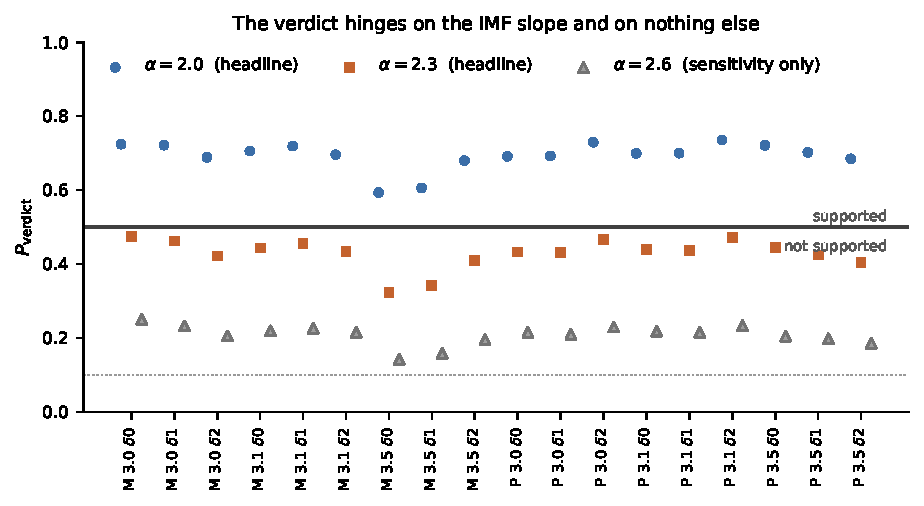
\includegraphics[width=\textwidth]{../figures/paper/fig6_verdict_branches.pdf}
\caption{$P_{\rm verdict}$ against every branch. The headline set
($\alpha = 2.0$ and $2.3$) is coloured and the sensitivity-only $\alpha = 2.6$
branches are grey; the solid line is the 0.5 support boundary and the dotted
line the 0.1 disfavour boundary of the pre-registered framing rule. Every
$\alpha = 2.0$ branch clears 0.5 and no $\alpha = 2.3$ branch does, with the
boundary falling precisely between the two slopes --- which is why the rule
returns \textsc{inconclusive} and what future work must settle.}
\label{fig:verdict}
\end{figure*}

The framing rule --- fixed at planning time and operationalized before the
number was known --- returns \textsc{inconclusive}, and hence this article
rather than a Letter.

\paragraph{Under the model's own permissive window.}
\citet{harer2025} themselves allow an event ``within the last few hundred
kyr''. Against that reading every branch clears 0.5,
$P = \Ppermlo$--\Ppermhi. The scenario is therefore \emph{supported} against
its authors' permissive statement and \emph{unresolved} against their preferred
$\sim$50\,kyr. Both windows were pre-registered before either was computed.

\subsection{$P \approx 0.5$ is a measurement, not a coin flip}

A coin returns 0.5 to every question. This analysis does not: it returns 0.055
for a 7\,kyr window, \Precent\ for 100\,kyr and \Ppermhi\ for the permissive
one. The relevant comparison is against ignorance. A last supernova distributed
uniformly over the association's \firstSN\,Myr active period would fall inside
100\,kyr with probability \ignorance; we measure \Precent, a factor of
\measurementFactor\ higher, because the rate is measured rather than assumed.
The number is near one half because the answer genuinely sits near the boundary,
not because the analysis is uninformative.

\subsection{Binary mass transfer, bounded}\label{sec:binary}

Our count is a single-star turnoff calculation, and most massive stars have
companions --- \citet{sana2012} find a close-binary fraction near 0.7 for
15--60\,$M_\odot$, and about two-thirds of Cygnus~OB2's own O and early-B stars
are resolved or spectroscopic multiples. Two independent lines bound what that omission costs.

Empirically, the BPASS \citep{stanway2018} calculation of \citet{harer2025}
--- \emph{with} binaries, for a population of the same mass and IMF slope --- gives a
core-collapse rate at 4\,Myr that is \bpassRatioLo--\bpassRatioHi\ times ours
once the difference in IMF integration ranges is corrected. The
binary-inclusive rate sits \emph{below} our single-star one, not above.
Theoretically, \citet{zapartas2017} find that binarity raises the integrated
number of core-collapse supernovae by $14^{+15}_{-14}$\%, but attribute the
increase to \emph{late} events, 50--200\,Myr after birth, from
4--8\,$M_\odot$ binaries, and find the early delay-time distributions
``remarkably similar'', diverging only around 20\,Myr. Cygnus~OB2 is 4\,Myr old
and its first supernova was \firstSN\,Myr ago, so the entire ledger sits inside
the regime where the two distributions agree, and the channel producing the
$+14$\% cannot have operated at all.

Nor does the living binary fraction translate directly. That
$30^{+10}_{-15}$\% of massive main-sequence stars are binary products
\citep{demink2014} is a statement about survivors: accretors and mergers are
rejuvenated, so a star pushed above the present turnoff by mass transfer has had
its clock partly reset and has typically \emph{not} yet exploded.

Adopting a deliberately conservative $\pm\binaryBracket$\% bracket --- the top
of the \citet{zapartas2017} enhancement applied in full despite its channel
being inapplicable --- and running it through the ledger engine moves the
baseline from \binaryLo\ to \binaryHi\ supernovae, a span of \binarySpan\
against a headline branch span of \branchSpan. \textbf{The systematic we do not
model is about \binaryRatio\ times smaller than the model-branch spread we do
report.} The upward arm helps the PeV-bubble scenario, so the verdict is
conservative with respect to it.

What binaries \emph{do} change is the supernova type, and there the effect is
already in the answer: $C_3 = \Cthree$. That does not smuggle binaries into the
result, because at 34--58\,$M_\odot$ single-star Wolf--Rayet winds strip
envelopes too, and Cygnus~OB2 contains three known WR stars.

\subsection{Systematics budget}\label{sec:systematics}

\paragraph{The absolute extinction scale.}
At matched sky position, prior-free broadband photometry prefers an $A_V$ about
0.5\,mag lower than the spectroscopically calibrated anchors
($p = 4.3\times10^{-16}$). The absolute extinction scale, and hence the mass
scale, the normalization and $N_{\rm SN}$, rests on the anchor calibration
rather than on the photometry alone. This is a systematic on the \emph{scale},
not on the relative structure: it moves all three subgroups together and does
not produce the A/B/C ordering. Its sign was checked and is the reassuring one
--- the anchors read \emph{higher}, the opposite of the failure mode in which a
selection-biased anchor set would drag the scale down.

\paragraph{Cyg~OB2-B's calibration asymmetry.}
B contains 4 spectroscopic anchors inside the member sample against 59 for A
and 42 for C, and its eighth-nearest anchor lies $0\fdg374$ away against
$0\fdg089$ and $0\fdg139$. Its extinction therefore rests on weaker local
calibration than its siblings'. This is an observational limitation of the
DR3-era anchor set, not a modelling choice: the kriging weights sum to 1.000 for
A and 0.992 for C but only 0.772 for B, so the correction is intrinsically
B-specific and no per-subgroup decision was made. The same fact surfaces three
times --- as B's extinction correction, as the last mass-function gate blocker,
and as B's age railing against its prior support.

\paragraph{B's age is a one-sided bound.}
\railB\% of B's counts-based age posterior sits on the topmost of its nine prior
nodes. A posterior that piles up against the edge of its prior grid reports a
bound, not a measurement, and the direction is known: older means a lower
turnoff means \emph{more} supernovae. Were B's true age the top node
(\railtopB\,Myr) its supernova count would rise by 15\%. B's contribution to
$N_{\rm SN}$ is therefore a lower bound at the precision quoted.

\paragraph{The in-situ fraction is an upper bound.}
The runaway count is a lower bound twice over --- the traceback is
two-dimensional, so line-of-sight ejections are missed, and the wide box caps
recovery at 44\,km\,s$^{-1}$ over 5\,Myr. A higher true runaway fraction lowers
$C_4$ and therefore the verdict. The effect is bounded: $C_4$ would have to fall
from \Cfour\ to below 0.60 to move any $\alpha = 2.0$ branch under 0.5. The
direction is against us and we state it.

\paragraph{Association mass, and which one.}
Three nested integrals of the same normalization can all be called ``the
association mass'', and they differ by a factor of 1.67. We quote the
multiplicity-adjusted stellar mass over 0.08--120\,$M_\odot$,
$\massTotal\times10^{4}\,M_\odot$. The like-for-like partner of
\citeauthor{wright2015}'s \citeyear{wright2015} $1.65\times10^{4}\,M_\odot$ ---
primary stars over the full range --- is $\massPrimaries\times10^{4}\,M_\odot$,
a factor \massVsWright. Integrating only 0.5--120\,$M_\odot$ instead gives
$\massPrimariesHalf\times10^{4}\,M_\odot$, which coincides with the literature
value but compares a different quantity. The comparison is an agreement at the
factor level, which is the resolution IMF-extrapolated cluster masses admit.

\subsection{Pre-registration as part of the result}

Every marker comparison in Sect.~\ref{sec:crosschecks} was pre-registered, with
its statistic and pass condition fixed, before the ledger it tests existed; the
markers themselves were frozen at data acquisition, before the normalization,
the census and the ledger were written. The question ``did you tune the analysis
to the markers?'' therefore has a checkable answer rather than a reassurance.
The same discipline produced results we would rather not have: predictions
recorded as failed and not reinterpreted, and two intermediate results withdrawn
after defects were found by comparison against externally known values
(Appendix~\ref{app:withdrawn}). We report this not as virtue but because the
verdict's credibility rests on it: an analysis that can be tuned to a
$\sim$50\,kyr window is not evidence about a $\sim$50\,kyr window.

\subsection{What \textit{Gaia}~DR4 will and will not fix}

DR4 improves three things that matter here: radial velocities for bright OB
stars make the traceback three-dimensional, so runaways stop being a lower bound
and $C_4$ tightens; better astrometry and photometry sharpen the subgroup ages,
including Cyg~OB2-C's family-dependent 2.52-versus-3.16\,Myr ambiguity and the
0--7 supernova range that follows from it; and deeper membership assigns
subgroups to the currently unlabelled massive members and orphan anchors. Gaia
XP spectra address Cyg~OB2-B's anchor famine specifically.

\textbf{DR4 will not settle the dominant term.} The verdict hinges on the
high-mass IMF slope, with a spread of \spreadAlpha\ against \spreadFamily\ for
everything astrometric. Distinguishing $\alpha = 2.0$ from $2.3$ needs a larger
or deeper massive-star census, or a second association analysed identically ---
not better astrometry on this one. We state the asymmetry because it is what
makes the forecast usable.

\subsection{Deferred}

Three questions are named here and left for later work rather than held against
this paper: a parallax-blind membership test, which is the only way to break the
circularity in our non-confirmation of the two-distance structure; a
distance-contamination test for Cyg~OB2-C, the leading explanation of its
closure excess; and the resolution of C's 0-versus-7 supernova family ambiguity,
which DR4 ages should settle.

%===============================================================
\section{Conclusions}\label{sec:conclusions}

\begin{enumerate}
\item Cygnus~OB2 resolves into three kinematic subgroups of \ageA, \ageB\ and
      \ageC\,Myr --- two older and one younger --- at $\ourDistance$\,kpc, with
      no evidence for two distinct distances among its members.
\item It has produced $N_{\rm SN} = \NSN$ supernovae on the baseline branch
      (median \NSNmedian, 68\% [\NSNlo, \NSNhi]), with a carried range of
      \NSNheadlo--\NSNheadhi\ across \NSNheadbranches\ branches. The first was
      \firstSN\,Myr ago; the most recent falls within the last 100\,kyr with
      probability \Precent.
\item The entire budget lies above $\bhSafeCut\,M_\odot$. For any black-hole
      threshold at or below that mass the ledger returns exactly zero on every
      branch, so the result is a measurement of very-massive-star
      explodability, and the 15--25\,$M_\odot$ island structure is irrelevant at
      this age.
\item PSR~J2032+4127 --- whose companion is a star in our own census --- settles
      that branch: a neutron star requires a successful explosion. Its age and
      kinematics agree with a ledger built without looking at it.
\item The census of stars above 8\,$M_\odot$ closes at $\alpha \approx 2.25$ and
      to \closureExcess\% at Salpeter, an out-of-sample validation of the IMF
      extrapolation that was deliberately not spent on selecting $\alpha$.
\item Applied to the supernova-driven interpretation of the Cygnus cocoon,
      $P = \Pverdictlo$--\Pverdicthi\ (median \Pverdictmed): supported on all
      $\alpha = 2.0$ branches, on no $\alpha = 2.3$ branch, and supported on
      every branch ($\Ppermlo$--\Ppermhi) under the model's own permissive age
      allowance. The verdict is a measurement, not a coin flip: against an
      ignorance baseline of \ignorance\ it is a factor
      \measurementFactor.
\item Unmodelled binary mass transfer is bounded at
      $\pm\binaryBracket$\% of $N_{\rm SN}$, about \binaryRatio\ times smaller
      than the branch spread already reported.
\end{enumerate}

\begin{acknowledgements}
This work has made use of data from the European Space Agency (ESA) mission
\textit{Gaia} (\url{https://www.cosmos.esa.int/gaia}), processed by the
\textit{Gaia} Data Processing and Analysis Consortium (DPAC,
\url{https://www.cosmos.esa.int/web/gaia/dpac/consortium}). Funding for the DPAC
has been provided by national institutions, in particular the institutions
participating in the \textit{Gaia} Multilateral Agreement. This publication
makes use of data products from the Two Micron All Sky Survey, and of NASA's
Astrophysics Data System.
\end{acknowledgements}

\bibliographystyle{aa}
\bibliography{references}

%===============================================================
\appendix

\section{Branches, gates and their verdicts}\label{app:branches}
% Table generated by scripts/wp10_numbers.py inputs; see
% tables/wp5_imf_norm_repair_v6.csv, tables/wp6_closure_repair_v7.csv,
% tables/wp7_ledger.csv, tables/wp9_verdict.csv.

\section{Provenance and reproducibility}\label{app:provenance}
Every cut, threshold, catalogue version and query is recorded with its date in
the project's provenance log, and every gate verdict exists as a
machine-readable record carrying SHA-256 digests of its inputs and outputs.
Nothing is overwritten: superseded artifacts are retained with version suffixes
and stay referenced. The manuscript's numbers are generated directly from those
artifacts; no number in this paper was typed by hand.

\section{Withdrawn and failed results}\label{app:withdrawn}
Two intermediate results were withdrawn after defects were found, both by
comparison against externally known values rather than by internal checks: a
runaway census computed from absolute rather than peculiar proper motions, and a
set of closure ratios whose forward integral was truncated at the same threshold
its response scatters across. Four pre-registered predictions were recorded as
failed and not reinterpreted. Both classes are listed here because a chain that
reports only its successes cannot be audited.

\end{document}
